\documentclass[twoside]{book}

% Packages required by doxygen
\usepackage{fixltx2e}
\usepackage{calc}
\usepackage{doxygen}
\usepackage[export]{adjustbox} % also loads graphicx
\usepackage{graphicx}
\usepackage[utf8]{inputenc}
\usepackage{makeidx}
\usepackage{multicol}
\usepackage{multirow}
\PassOptionsToPackage{warn}{textcomp}
\usepackage{textcomp}
\usepackage[nointegrals]{wasysym}
\usepackage[table]{xcolor}

% Font selection
\usepackage[T1]{fontenc}
\usepackage[scaled=.90]{helvet}
\usepackage{courier}
\usepackage{amssymb}
\usepackage{sectsty}
\renewcommand{\familydefault}{\sfdefault}
\allsectionsfont{%
  \fontseries{bc}\selectfont%
  \color{darkgray}%
}
\renewcommand{\DoxyLabelFont}{%
  \fontseries{bc}\selectfont%
  \color{darkgray}%
}
\newcommand{\+}{\discretionary{\mbox{\scriptsize$\hookleftarrow$}}{}{}}

% Page & text layout
\usepackage{geometry}
\geometry{%
  a4paper,%
  top=2.5cm,%
  bottom=2.5cm,%
  left=2.5cm,%
  right=2.5cm%
}
\tolerance=750
\hfuzz=15pt
\hbadness=750
\setlength{\emergencystretch}{15pt}
\setlength{\parindent}{0cm}
\setlength{\parskip}{3ex plus 2ex minus 2ex}
\makeatletter
\renewcommand{\paragraph}{%
  \@startsection{paragraph}{4}{0ex}{-1.0ex}{1.0ex}{%
    \normalfont\normalsize\bfseries\SS@parafont%
  }%
}
\renewcommand{\subparagraph}{%
  \@startsection{subparagraph}{5}{0ex}{-1.0ex}{1.0ex}{%
    \normalfont\normalsize\bfseries\SS@subparafont%
  }%
}
\makeatother

% Headers & footers
\usepackage{fancyhdr}
\pagestyle{fancyplain}
\fancyhead[LE]{\fancyplain{}{\bfseries\thepage}}
\fancyhead[CE]{\fancyplain{}{}}
\fancyhead[RE]{\fancyplain{}{\bfseries\leftmark}}
\fancyhead[LO]{\fancyplain{}{\bfseries\rightmark}}
\fancyhead[CO]{\fancyplain{}{}}
\fancyhead[RO]{\fancyplain{}{\bfseries\thepage}}
\fancyfoot[LE]{\fancyplain{}{}}
\fancyfoot[CE]{\fancyplain{}{}}
\fancyfoot[RE]{\fancyplain{}{\bfseries\scriptsize Generated by Doxygen }}
\fancyfoot[LO]{\fancyplain{}{\bfseries\scriptsize Generated by Doxygen }}
\fancyfoot[CO]{\fancyplain{}{}}
\fancyfoot[RO]{\fancyplain{}{}}
\renewcommand{\footrulewidth}{0.4pt}
\renewcommand{\chaptermark}[1]{%
  \markboth{#1}{}%
}
\renewcommand{\sectionmark}[1]{%
  \markright{\thesection\ #1}%
}

% Indices & bibliography
\usepackage{natbib}
\usepackage[titles]{tocloft}
\setcounter{tocdepth}{3}
\setcounter{secnumdepth}{5}
\makeindex

% Hyperlinks (required, but should be loaded last)
\usepackage{ifpdf}
\ifpdf
  \usepackage[pdftex,pagebackref=true]{hyperref}
\else
  \usepackage[ps2pdf,pagebackref=true]{hyperref}
\fi
\hypersetup{%
  colorlinks=true,%
  linkcolor=blue,%
  citecolor=blue,%
  unicode%
}

% Custom commands
\newcommand{\clearemptydoublepage}{%
  \newpage{\pagestyle{empty}\cleardoublepage}%
}

\usepackage{caption}
\captionsetup{labelsep=space,justification=centering,font={bf},singlelinecheck=off,skip=4pt,position=top}

%===== C O N T E N T S =====

\begin{document}

% Titlepage & ToC
\hypersetup{pageanchor=false,
             bookmarksnumbered=true,
             pdfencoding=unicode
            }
\pagenumbering{alph}
\begin{titlepage}
\vspace*{7cm}
\begin{center}%
{\Large C\+R\+TS \\[1ex]\large Version 0.\+3 }\\
\vspace*{1cm}
{\large Generated by Doxygen 1.8.13}\\
\end{center}
\end{titlepage}
\clearemptydoublepage
\pagenumbering{roman}
\tableofcontents
\clearemptydoublepage
\pagenumbering{arabic}
\hypersetup{pageanchor=true}

%--- Begin generated contents ---
\chapter{Todo List}
\label{todo}
\Hypertarget{todo}

\begin{DoxyRefList}
\item[\label{todo__todo000002}%
\Hypertarget{todo__todo000002}%
Member \hyperlink{classCRTSController_aa2b26a62c62fe5758ab5cc9104e96b56}{C\+R\+T\+S\+Controller\+:\+:get\+Control} (const std\+::string name=\char`\"{}\char`\"{}, bool add\+Controller=true, bool start=false)]add example code. 
\item[\label{todo__todo000001}%
\Hypertarget{todo__todo000001}%
Member \hyperlink{classCRTSFilter_acc17d29240468c94e360e1b788f5d6a0}{C\+R\+T\+S\+Filter\+:\+:add\+Parameter} (std\+::string name, std\+::function$<$ double(void)$>$ get, std\+::function$<$ bool(const double \&)$>$ set=0, bool over\+Write=false)]doubles can be converted to many other types, but a double can\textquotesingle{}t be made into any type. If we template out the double we\textquotesingle{}ll lose the seamless nature of this control interface, or will we.
\end{DoxyRefList}
\chapter{Class Index}
\section{Class List}
Here are the classes, structs, unions and interfaces with brief descriptions\+:\begin{DoxyCompactList}
\item\contentsline{section}{\hyperlink{classCRTSControl}{C\+R\+T\+S\+Control} }{\pageref{classCRTSControl}}{}
\item\contentsline{section}{\hyperlink{classCRTSController}{C\+R\+T\+S\+Controller} }{\pageref{classCRTSController}}{}
\item\contentsline{section}{\hyperlink{classCRTSFilter}{C\+R\+T\+S\+Filter} }{\pageref{classCRTSFilter}}{}
\item\contentsline{section}{\hyperlink{classCRTSStream}{C\+R\+T\+S\+Stream} }{\pageref{classCRTSStream}}{}
\end{DoxyCompactList}

\chapter{Class Documentation}
\hypertarget{classCRTSControl}{}\section{C\+R\+T\+S\+Control Class Reference}
\label{classCRTSControl}\index{C\+R\+T\+S\+Control@{C\+R\+T\+S\+Control}}


{\ttfamily \#include $<$Filter.\+hpp$>$}



Collaboration diagram for C\+R\+T\+S\+Control\+:
\nopagebreak
\begin{figure}[H]
\begin{center}
\leavevmode
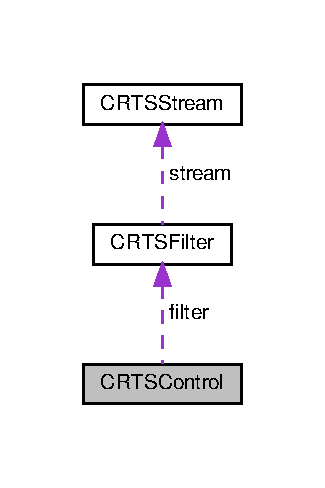
\includegraphics[width=156pt]{classCRTSControl__coll__graph}
\end{center}
\end{figure}
\subsection*{Public Member Functions}
\begin{DoxyCompactItemize}
\item 
uint64\+\_\+t \hyperlink{classCRTSControl_ad9acd9abb7620a0b34b724b26a47740d}{total\+Bytes\+In} (uint32\+\_\+t in\+Channel\+Num=\hyperlink{classCRTSFilter_a9ea354654e8e2e8ce3bff293cc35fafe}{C\+R\+T\+S\+Filter\+::\+A\+L\+L\+\_\+\+C\+H\+A\+N\+N\+E\+LS}) const
\item 
uint64\+\_\+t \hyperlink{classCRTSControl_ae39f48f9761149fabebe68870ec2b8b8}{total\+Bytes\+Out} (uint32\+\_\+t out\+Channel\+Num=\hyperlink{classCRTSFilter_a9ea354654e8e2e8ce3bff293cc35fafe}{C\+R\+T\+S\+Filter\+::\+A\+L\+L\+\_\+\+C\+H\+A\+N\+N\+E\+LS}) const
\item 
std\+::string \hyperlink{classCRTSControl_a493557760b3354b32de76fc9f60feaed}{get\+Next\+Parameter\+Name} (bool start=false, bool $\ast$has\+Set=0, bool $\ast$has\+Get=0)
\item 
void \hyperlink{classCRTSControl_aca9bf2af70e093eb050f1b964594c9ec}{get\+Parameter} (const std\+::string pname, std\+::function$<$ void(double)$>$ callback)
\item 
double \hyperlink{classCRTSControl_a49b888b6fb53ca9f407b227cc6c93d9b}{get\+Parameter} (const std\+::string pname)
\item 
bool \hyperlink{classCRTSControl_a80591c5f74bac27c33662884dfaa06ac}{set\+Parameter} (const std\+::string pname, const double \&val) const
\item 
void \hyperlink{classCRTSControl_a1cbcd31c134d09cb2619fde63e064727}{add\+Controller} (\hyperlink{classCRTSController}{C\+R\+T\+S\+Controller} $\ast$controller)
\item 
uint32\+\_\+t \hyperlink{classCRTSControl_acfb6005cbc2d5f22fd4703283c9636bd}{get\+Id} (void) const
\end{DoxyCompactItemize}


\subsection{Detailed Description}
The C\+R\+T\+S\+Controls should be accessed in the \hyperlink{classCRTSFilter}{C\+R\+T\+S\+Filter} thread that it is associated with or in the main thread in a constructor.

C\+R\+T\+S\+Controls is a factory of any number of Parameters. 

\subsection{Member Function Documentation}
\mbox{\Hypertarget{classCRTSControl_a1cbcd31c134d09cb2619fde63e064727}\label{classCRTSControl_a1cbcd31c134d09cb2619fde63e064727}} 
\index{C\+R\+T\+S\+Control@{C\+R\+T\+S\+Control}!add\+Controller@{add\+Controller}}
\index{add\+Controller@{add\+Controller}!C\+R\+T\+S\+Control@{C\+R\+T\+S\+Control}}
\subsubsection{\texorpdfstring{add\+Controller()}{addController()}}
{\footnotesize\ttfamily void C\+R\+T\+S\+Control\+::add\+Controller (\begin{DoxyParamCaption}\item[{\hyperlink{classCRTSController}{C\+R\+T\+S\+Controller} $\ast$}]{controller }\end{DoxyParamCaption})\hspace{0.3cm}{\ttfamily [inline]}}

Add a controller to a filter control callback list.

This will cause the \hyperlink{classCRTSController_af9d93f0eee3c2d0969c6aaaaf94eb839}{C\+R\+T\+S\+Controller\+::execute()} to be called before every \hyperlink{classCRTSFilter_ab75eb3db5914c0d6b3781439d46b2301}{C\+R\+T\+S\+Filter\+::input()}.

/param controller a pointer to the \hyperlink{classCRTSController}{C\+R\+T\+S\+Controller} object. \mbox{\Hypertarget{classCRTSControl_acfb6005cbc2d5f22fd4703283c9636bd}\label{classCRTSControl_acfb6005cbc2d5f22fd4703283c9636bd}} 
\index{C\+R\+T\+S\+Control@{C\+R\+T\+S\+Control}!get\+Id@{get\+Id}}
\index{get\+Id@{get\+Id}!C\+R\+T\+S\+Control@{C\+R\+T\+S\+Control}}
\subsubsection{\texorpdfstring{get\+Id()}{getId()}}
{\footnotesize\ttfamily uint32\+\_\+t C\+R\+T\+S\+Control\+::get\+Id (\begin{DoxyParamCaption}\item[{void}]{ }\end{DoxyParamCaption}) const\hspace{0.3cm}{\ttfamily [inline]}}

/return unique ID that can be quickly used to distinguish this \hyperlink{classCRTSControl}{C\+R\+T\+S\+Control} from other C\+R\+T\+S\+Controls in this \hyperlink{classCRTSFilter}{C\+R\+T\+S\+Filter}. \mbox{\Hypertarget{classCRTSControl_a493557760b3354b32de76fc9f60feaed}\label{classCRTSControl_a493557760b3354b32de76fc9f60feaed}} 
\index{C\+R\+T\+S\+Control@{C\+R\+T\+S\+Control}!get\+Next\+Parameter\+Name@{get\+Next\+Parameter\+Name}}
\index{get\+Next\+Parameter\+Name@{get\+Next\+Parameter\+Name}!C\+R\+T\+S\+Control@{C\+R\+T\+S\+Control}}
\subsubsection{\texorpdfstring{get\+Next\+Parameter\+Name()}{getNextParameterName()}}
{\footnotesize\ttfamily std\+::string C\+R\+T\+S\+Control\+::get\+Next\+Parameter\+Name (\begin{DoxyParamCaption}\item[{bool}]{start = {\ttfamily false},  }\item[{bool $\ast$}]{has\+Set = {\ttfamily 0},  }\item[{bool $\ast$}]{has\+Get = {\ttfamily 0} }\end{DoxyParamCaption})\hspace{0.3cm}{\ttfamily [inline]}}

Get information about parameters in this \hyperlink{classCRTSControl}{C\+R\+T\+S\+Control}

Iterates through all the parameters in this control getting the name and optionally whither there is a setter and a getter function for this parameter.


\begin{DoxyParams}{Parameters}
{\em start} & if set this will start at the beginning of the list of parameters in this \hyperlink{classCRTSControl}{C\+R\+T\+S\+Control}. The first time this is called by a \hyperlink{classCRTSController}{C\+R\+T\+S\+Controller} {\itshape start} should be true.\\
\hline
{\em has\+Set} & if set the value that this points to will get set to true if there is a setter function for this parameter, or it will get set to false otherwise.\\
\hline
{\em has\+Get} & if set the value that this points to will get set to true if there is a getter function for this parameter, or it will get set to false otherwise.\\
\hline
\end{DoxyParams}
\begin{DoxyReturn}{Returns}
a std\+::string that is the name of this parameter. If the returned string is empty than we are at the end of the list of parameters. 
\end{DoxyReturn}
\mbox{\Hypertarget{classCRTSControl_aca9bf2af70e093eb050f1b964594c9ec}\label{classCRTSControl_aca9bf2af70e093eb050f1b964594c9ec}} 
\index{C\+R\+T\+S\+Control@{C\+R\+T\+S\+Control}!get\+Parameter@{get\+Parameter}}
\index{get\+Parameter@{get\+Parameter}!C\+R\+T\+S\+Control@{C\+R\+T\+S\+Control}}
\subsubsection{\texorpdfstring{get\+Parameter()}{getParameter()}\hspace{0.1cm}{\footnotesize\ttfamily [1/2]}}
{\footnotesize\ttfamily void C\+R\+T\+S\+Control\+::get\+Parameter (\begin{DoxyParamCaption}\item[{const std\+::string}]{pname,  }\item[{std\+::function$<$ void(double)$>$}]{callback }\end{DoxyParamCaption})\hspace{0.3cm}{\ttfamily [inline]}}

Set a callback that gets a parameter value from the \hyperlink{classCRTSFilter}{C\+R\+T\+S\+Filter} that this \hyperlink{classCRTSControl}{C\+R\+T\+S\+Control} is associated with.

The callback will be called when the stream is flowing. The callback will be called in the in the filter\textquotesingle{}s thread, before or during the filter\textquotesingle{}s input() is called. So this callback is associated with a particular filter that owns this \hyperlink{classCRTSControl}{C\+R\+T\+S\+Control}.

/param callback function that is called any time that the parameter changes. \mbox{\Hypertarget{classCRTSControl_a49b888b6fb53ca9f407b227cc6c93d9b}\label{classCRTSControl_a49b888b6fb53ca9f407b227cc6c93d9b}} 
\index{C\+R\+T\+S\+Control@{C\+R\+T\+S\+Control}!get\+Parameter@{get\+Parameter}}
\index{get\+Parameter@{get\+Parameter}!C\+R\+T\+S\+Control@{C\+R\+T\+S\+Control}}
\subsubsection{\texorpdfstring{get\+Parameter()}{getParameter()}\hspace{0.1cm}{\footnotesize\ttfamily [2/2]}}
{\footnotesize\ttfamily double C\+R\+T\+S\+Control\+::get\+Parameter (\begin{DoxyParamCaption}\item[{const std\+::string}]{pname }\end{DoxyParamCaption})\hspace{0.3cm}{\ttfamily [inline]}}

Get a parameter value from the \hyperlink{classCRTSFilter}{C\+R\+T\+S\+Filter} that this \hyperlink{classCRTSControl}{C\+R\+T\+S\+Control} is associated with.

/param pname the name of the parameter that we seek.

/return the value of the parameter as a double. If the parameter with the name {\ttfamily pname} was not found, {\itshape N\+AN} is returned. \mbox{\Hypertarget{classCRTSControl_a80591c5f74bac27c33662884dfaa06ac}\label{classCRTSControl_a80591c5f74bac27c33662884dfaa06ac}} 
\index{C\+R\+T\+S\+Control@{C\+R\+T\+S\+Control}!set\+Parameter@{set\+Parameter}}
\index{set\+Parameter@{set\+Parameter}!C\+R\+T\+S\+Control@{C\+R\+T\+S\+Control}}
\subsubsection{\texorpdfstring{set\+Parameter()}{setParameter()}}
{\footnotesize\ttfamily bool C\+R\+T\+S\+Control\+::set\+Parameter (\begin{DoxyParamCaption}\item[{const std\+::string}]{pname,  }\item[{const double \&}]{val }\end{DoxyParamCaption}) const\hspace{0.3cm}{\ttfamily [inline]}}

Set a parameter value from the \hyperlink{classCRTSFilter}{C\+R\+T\+S\+Filter} that this \hyperlink{classCRTSControl}{C\+R\+T\+S\+Control} is associated with.

/todo make a object set(pname) with method that uses operator \textquotesingle{}=\textquotesingle{}. Like set\mbox{[}\char`\"{}freq\char`\"{}\mbox{]}

This should only be called in the excute() function which is passed this \hyperlink{classCRTSControl}{C\+R\+T\+S\+Control}. This will run filters input() thread before input() is called.

/param pname the name of the parameter that we seek to set.

/param val the value we wish to set the parameter to.

/return true is this call affected the parameter. \mbox{\Hypertarget{classCRTSControl_ad9acd9abb7620a0b34b724b26a47740d}\label{classCRTSControl_ad9acd9abb7620a0b34b724b26a47740d}} 
\index{C\+R\+T\+S\+Control@{C\+R\+T\+S\+Control}!total\+Bytes\+In@{total\+Bytes\+In}}
\index{total\+Bytes\+In@{total\+Bytes\+In}!C\+R\+T\+S\+Control@{C\+R\+T\+S\+Control}}
\subsubsection{\texorpdfstring{total\+Bytes\+In()}{totalBytesIn()}}
{\footnotesize\ttfamily uint64\+\_\+t C\+R\+T\+S\+Control\+::total\+Bytes\+In (\begin{DoxyParamCaption}\item[{uint32\+\_\+t}]{in\+Channel\+Num = {\ttfamily \hyperlink{classCRTSFilter_a9ea354654e8e2e8ce3bff293cc35fafe}{C\+R\+T\+S\+Filter\+::\+A\+L\+L\+\_\+\+C\+H\+A\+N\+N\+E\+LS}} }\end{DoxyParamCaption}) const\hspace{0.3cm}{\ttfamily [inline]}}

/param in\+Channel\+Num the channel number that the \hyperlink{classCRTSFilter}{C\+R\+T\+S\+Filter} is referring to.

/return the total number of bytes that the associated input channel have been consumed by the associated \hyperlink{classCRTSFilter}{C\+R\+T\+S\+Filter} since the last start. \mbox{\Hypertarget{classCRTSControl_ae39f48f9761149fabebe68870ec2b8b8}\label{classCRTSControl_ae39f48f9761149fabebe68870ec2b8b8}} 
\index{C\+R\+T\+S\+Control@{C\+R\+T\+S\+Control}!total\+Bytes\+Out@{total\+Bytes\+Out}}
\index{total\+Bytes\+Out@{total\+Bytes\+Out}!C\+R\+T\+S\+Control@{C\+R\+T\+S\+Control}}
\subsubsection{\texorpdfstring{total\+Bytes\+Out()}{totalBytesOut()}}
{\footnotesize\ttfamily uint64\+\_\+t C\+R\+T\+S\+Control\+::total\+Bytes\+Out (\begin{DoxyParamCaption}\item[{uint32\+\_\+t}]{out\+Channel\+Num = {\ttfamily \hyperlink{classCRTSFilter_a9ea354654e8e2e8ce3bff293cc35fafe}{C\+R\+T\+S\+Filter\+::\+A\+L\+L\+\_\+\+C\+H\+A\+N\+N\+E\+LS}} }\end{DoxyParamCaption}) const\hspace{0.3cm}{\ttfamily [inline]}}

/param out\+Channel\+Num the channel number that the \hyperlink{classCRTSFilter}{C\+R\+T\+S\+Filter} is referring to.

/return the total number of bytes that the associated output channel have been pushed to the associated \hyperlink{classCRTSFilter}{C\+R\+T\+S\+Filter} that is connected since the last start.

This may not be the same as the number of bytes consumed, \hyperlink{classCRTSControl_ad9acd9abb7620a0b34b724b26a47740d}{total\+Bytes\+In()}, by the connected \hyperlink{classCRTSFilter}{C\+R\+T\+S\+Filter}, because there may be data queued up and the connected \hyperlink{classCRTSFilter}{C\+R\+T\+S\+Filter} may be waiting for a certain amount or type of data before it marks the data as consumed. 

The documentation for this class was generated from the following file\+:\begin{DoxyCompactItemize}
\item 
/home/progb/git/crts/include/crts/Filter.\+hpp\end{DoxyCompactItemize}

\hypertarget{classCRTSController}{}\section{C\+R\+T\+S\+Controller Class Reference}
\label{classCRTSController}\index{C\+R\+T\+S\+Controller@{C\+R\+T\+S\+Controller}}


{\ttfamily \#include $<$Filter.\+hpp$>$}

\subsection*{Public Member Functions}
\begin{DoxyCompactItemize}
\item 
virtual void \hyperlink{classCRTSController_a9065844e7c7aac10e26dad339ee65a8c}{start} (\hyperlink{classCRTSControl}{C\+R\+T\+S\+Control} $\ast$c, uint32\+\_\+t num\+Channels\+In, uint32\+\_\+t num\+Channels\+Out)
\item 
virtual void \hyperlink{classCRTSController_a883c09ddb21374753c3be0fc66f016fb}{stop} (\hyperlink{classCRTSControl}{C\+R\+T\+S\+Control} $\ast$c)
\item 
virtual void \hyperlink{classCRTSController_af9d93f0eee3c2d0969c6aaaaf94eb839}{execute} (\hyperlink{classCRTSControl}{C\+R\+T\+S\+Control} $\ast$c, const void $\ast$buffer, size\+\_\+t len, uint32\+\_\+t channel\+Num)=0
\item 
bool \hyperlink{classCRTSController_a7b167f03af923a194efecfc551015087}{print\+Stream\+Graph\+Dot\+P\+N\+G64} (int fd)
\end{DoxyCompactItemize}
\subsection*{Protected Member Functions}
\begin{DoxyCompactItemize}
\item 
{\footnotesize template$<$class C $>$ }\\C \hyperlink{classCRTSController_aa2b26a62c62fe5758ab5cc9104e96b56}{get\+Control} (const std\+::string name=\char`\"{}\char`\"{}, bool add\+Controller=true, bool \hyperlink{classCRTSController_a9065844e7c7aac10e26dad339ee65a8c}{start}=false)
\end{DoxyCompactItemize}


\subsection{Detailed Description}
A Controller module base class

Used to monitor and control the filter flow stream by setting and getting \hyperlink{classCRTSFilter}{C\+R\+T\+S\+Filter} parameters, and directly executing code before inputting data chunks into filters. 

\subsection{Member Function Documentation}
\mbox{\Hypertarget{classCRTSController_af9d93f0eee3c2d0969c6aaaaf94eb839}\label{classCRTSController_af9d93f0eee3c2d0969c6aaaaf94eb839}} 
\index{C\+R\+T\+S\+Controller@{C\+R\+T\+S\+Controller}!execute@{execute}}
\index{execute@{execute}!C\+R\+T\+S\+Controller@{C\+R\+T\+S\+Controller}}
\subsubsection{\texorpdfstring{execute()}{execute()}}
{\footnotesize\ttfamily virtual void C\+R\+T\+S\+Controller\+::execute (\begin{DoxyParamCaption}\item[{\hyperlink{classCRTSControl}{C\+R\+T\+S\+Control} $\ast$}]{c,  }\item[{const void $\ast$}]{buffer,  }\item[{size\+\_\+t}]{len,  }\item[{uint32\+\_\+t}]{channel\+Num }\end{DoxyParamCaption})\hspace{0.3cm}{\ttfamily [pure virtual]}}

execute is called before each \hyperlink{classCRTSFilter}{C\+R\+T\+S\+Filter} that owns the \hyperlink{classCRTSControl}{C\+R\+T\+S\+Control} calls output() for the connected C\+R\+T\+S\+Filters.

When this is called, we are running in the \hyperlink{classCRTSFilter}{C\+R\+T\+S\+Filter} that owns the \hyperlink{classCRTSControl}{C\+R\+T\+S\+Control} that is passed in. We can\textquotesingle{}t used controls from other \hyperlink{classCRTSFilter}{C\+R\+T\+S\+Filter} objects, because they may be accessed in other threads.

This is the only method that that is not called from the main thread. All other methods are called in the main thread.

/param c the \hyperlink{classCRTSControl}{C\+R\+T\+S\+Control} that is owned by the \hyperlink{classCRTSFilter}{C\+R\+T\+S\+Filter} that called this.

/param buffer pointer to the next list of bytes that will come into the \hyperlink{classCRTSFilter}{C\+R\+T\+S\+Filter} that receive this data.

/param len length of data that could be read, but may not necessarily be read after this call.

/param channel\+Num the C\+R\+T\+S\+Filters channel number that it uses to refer to the connection in the filter stream. \mbox{\Hypertarget{classCRTSController_aa2b26a62c62fe5758ab5cc9104e96b56}\label{classCRTSController_aa2b26a62c62fe5758ab5cc9104e96b56}} 
\index{C\+R\+T\+S\+Controller@{C\+R\+T\+S\+Controller}!get\+Control@{get\+Control}}
\index{get\+Control@{get\+Control}!C\+R\+T\+S\+Controller@{C\+R\+T\+S\+Controller}}
\subsubsection{\texorpdfstring{get\+Control()}{getControl()}}
{\footnotesize\ttfamily template$<$class C $>$ \\
C C\+R\+T\+S\+Controller\+::get\+Control (\begin{DoxyParamCaption}\item[{const std\+::string}]{name = {\ttfamily \char`\"{}\char`\"{}},  }\item[{bool}]{add\+Controller = {\ttfamily true},  }\item[{bool}]{start = {\ttfamily false} }\end{DoxyParamCaption})\hspace{0.3cm}{\ttfamily [protected]}}

Returns 0 if the control with name name was not found in the list of all C\+R\+TS controls. The particular \hyperlink{classCRTSController}{C\+R\+T\+S\+Controller} can get pointers to any \hyperlink{classCRTSControl}{C\+R\+T\+S\+Control} objects.

You do not need to (or want to) delete the \hyperlink{classCRTSControl}{C\+R\+T\+S\+Control} object that this points to. It is managed by the associated \hyperlink{classCRTSFilter}{C\+R\+T\+S\+Filter} object.

This must be called in the main thread in \hyperlink{classCRTSController_a9065844e7c7aac10e26dad339ee65a8c}{start()} or \hyperlink{classCRTSController_a883c09ddb21374753c3be0fc66f016fb}{stop()}.

The \hyperlink{classCRTSController}{C\+R\+T\+S\+Controller} implementation must include the particular \hyperlink{classCRTSFilter}{C\+R\+T\+S\+Filter} interface header file to get access to the control methods that are implemented.

\begin{DoxyRefDesc}{Todo}
\item[\hyperlink{todo__todo000002}{Todo}]add example code.\end{DoxyRefDesc}



\begin{DoxyParams}{Parameters}
{\em name} & the unique (across the \hyperlink{classCRTSStream}{C\+R\+T\+S\+Stream}) name of this \hyperlink{classCRTSControl}{C\+R\+T\+S\+Control}. If name is an empty string than this will iterate through all controls returning them in std\+::map iterated order and return 0 at the end.\\
\hline
\end{DoxyParams}
\begin{DoxyReturn}{Returns}
a \hyperlink{classCRTSControl}{C\+R\+T\+S\+Control} object pointer. 
\end{DoxyReturn}
\mbox{\Hypertarget{classCRTSController_a7b167f03af923a194efecfc551015087}\label{classCRTSController_a7b167f03af923a194efecfc551015087}} 
\index{C\+R\+T\+S\+Controller@{C\+R\+T\+S\+Controller}!print\+Stream\+Graph\+Dot\+P\+N\+G64@{print\+Stream\+Graph\+Dot\+P\+N\+G64}}
\index{print\+Stream\+Graph\+Dot\+P\+N\+G64@{print\+Stream\+Graph\+Dot\+P\+N\+G64}!C\+R\+T\+S\+Controller@{C\+R\+T\+S\+Controller}}
\subsubsection{\texorpdfstring{print\+Stream\+Graph\+Dot\+P\+N\+G64()}{printStreamGraphDotPNG64()}}
{\footnotesize\ttfamily bool C\+R\+T\+S\+Controller\+::print\+Stream\+Graph\+Dot\+P\+N\+G64 (\begin{DoxyParamCaption}\item[{int}]{fd }\end{DoxyParamCaption})}

print the stream graph image to a file descriptor

For example\+: we use this to send a base 64 encoded P\+NG image to a socket.


\begin{DoxyParams}{Parameters}
{\em fd} & is the file descriptor to write the P\+NG file to.\\
\hline
\end{DoxyParams}
\begin{DoxyReturn}{Returns}
false on success and true on error. This will spew on error. 
\end{DoxyReturn}
\mbox{\Hypertarget{classCRTSController_a9065844e7c7aac10e26dad339ee65a8c}\label{classCRTSController_a9065844e7c7aac10e26dad339ee65a8c}} 
\index{C\+R\+T\+S\+Controller@{C\+R\+T\+S\+Controller}!start@{start}}
\index{start@{start}!C\+R\+T\+S\+Controller@{C\+R\+T\+S\+Controller}}
\subsubsection{\texorpdfstring{start()}{start()}}
{\footnotesize\ttfamily virtual void C\+R\+T\+S\+Controller\+::start (\begin{DoxyParamCaption}\item[{\hyperlink{classCRTSControl}{C\+R\+T\+S\+Control} $\ast$}]{c,  }\item[{uint32\+\_\+t}]{num\+Channels\+In,  }\item[{uint32\+\_\+t}]{num\+Channels\+Out }\end{DoxyParamCaption})\hspace{0.3cm}{\ttfamily [inline]}, {\ttfamily [virtual]}}

start is called after all the filters start and before the stream is running.

A module class that inherits \hyperlink{classCRTSController}{C\+R\+T\+S\+Controller} may opt out of writing a \hyperlink{classCRTSController_a9065844e7c7aac10e26dad339ee65a8c}{start()} method.

/param num\+Channels\+In is the number of channels that input into this filter with this \hyperlink{classCRTSControl}{C\+R\+T\+S\+Control}.

/param num\+Channels\+Out is the number of channels that will output from this filter with this \hyperlink{classCRTSControl}{C\+R\+T\+S\+Control}.

/param c the filters C\+R\+TS control \mbox{\Hypertarget{classCRTSController_a883c09ddb21374753c3be0fc66f016fb}\label{classCRTSController_a883c09ddb21374753c3be0fc66f016fb}} 
\index{C\+R\+T\+S\+Controller@{C\+R\+T\+S\+Controller}!stop@{stop}}
\index{stop@{stop}!C\+R\+T\+S\+Controller@{C\+R\+T\+S\+Controller}}
\subsubsection{\texorpdfstring{stop()}{stop()}}
{\footnotesize\ttfamily virtual void C\+R\+T\+S\+Controller\+::stop (\begin{DoxyParamCaption}\item[{\hyperlink{classCRTSControl}{C\+R\+T\+S\+Control} $\ast$}]{c }\end{DoxyParamCaption})\hspace{0.3cm}{\ttfamily [inline]}, {\ttfamily [virtual]}}

stop is called just before the filters stop.

A module class that inherits \hyperlink{classCRTSController}{C\+R\+T\+S\+Controller} may opt out of writing a \hyperlink{classCRTSController_a883c09ddb21374753c3be0fc66f016fb}{stop()} method.

/param c the filters C\+R\+TS control 

The documentation for this class was generated from the following file\+:\begin{DoxyCompactItemize}
\item 
/home/progb/git/crts/include/crts/Filter.\+hpp\end{DoxyCompactItemize}

\hypertarget{classCRTSFilter}{}\section{C\+R\+T\+S\+Filter Class Reference}
\label{classCRTSFilter}\index{C\+R\+T\+S\+Filter@{C\+R\+T\+S\+Filter}}


{\ttfamily \#include $<$Filter.\+hpp$>$}



Collaboration diagram for C\+R\+T\+S\+Filter\+:
\nopagebreak
\begin{figure}[H]
\begin{center}
\leavevmode
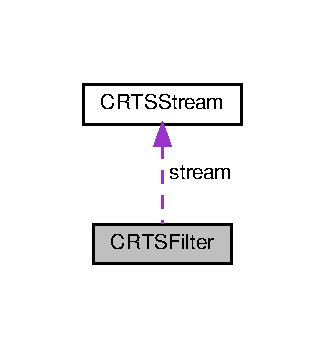
\includegraphics[width=156pt]{classCRTSFilter__coll__graph}
\end{center}
\end{figure}
\subsection*{Public Member Functions}
\begin{DoxyCompactItemize}
\item 
virtual void \hyperlink{classCRTSFilter_ab75eb3db5914c0d6b3781439d46b2301}{input} (void $\ast$buffer, size\+\_\+t buffer\+Len, uint32\+\_\+t input\+Channel\+Num)=0
\item 
virtual bool \hyperlink{classCRTSFilter_a15a3e99b38a67fd40559776d468b95fa}{start} (uint32\+\_\+t num\+Input\+Channels, uint32\+\_\+t num\+Output\+Channels)
\item 
virtual bool \hyperlink{classCRTSFilter_a934e38c5cd6bd82b309166180f664f0c}{stop} (uint32\+\_\+t num\+Input\+Channels, uint32\+\_\+t num\+Output\+Channels)
\item 
\hyperlink{classCRTSFilter_a2d907e8b7d986f35a5cb31171f7d683f}{C\+R\+T\+S\+Filter} (std\+::string control\+Name=\char`\"{}\char`\"{})
\end{DoxyCompactItemize}
\subsection*{Public Attributes}
\begin{DoxyCompactItemize}
\item 
\hyperlink{classCRTSStream}{C\+R\+T\+S\+Stream} $\ast$ \hyperlink{classCRTSFilter_aa6986d6a10ed56ea4af4ebcf41337e73}{stream}
\end{DoxyCompactItemize}
\subsection*{Static Public Attributes}
\begin{DoxyCompactItemize}
\item 
static const uint32\+\_\+t \hyperlink{classCRTSFilter_a9ea354654e8e2e8ce3bff293cc35fafe}{A\+L\+L\+\_\+\+C\+H\+A\+N\+N\+E\+LS}
\item 
static const uint32\+\_\+t \hyperlink{classCRTSFilter_af731176aa73539af3cfc69b6c1051f82}{N\+U\+L\+L\+\_\+\+C\+H\+A\+N\+N\+EL}
\end{DoxyCompactItemize}
\subsection*{Protected Member Functions}
\begin{DoxyCompactItemize}
\item 
bool \hyperlink{classCRTSFilter_acacdf624ab19ae5ad6394a647dccc353}{is\+Source} (void)
\item 
void \hyperlink{classCRTSFilter_a7898d77d1a5acbadb45769eff2a01cfb}{advance\+Input} (size\+\_\+t len)
\item 
bool \hyperlink{classCRTSFilter_a33ee2e0151f822aec425d6d22ab94757}{set\+Parameter} (const std\+::string name, double value)
\item 
void \hyperlink{classCRTSFilter_a7a10a3daf1d7ee26e8b414c16901b315}{create\+Output\+Buffer} (size\+\_\+t max\+Length, uint32\+\_\+t output\+Channel\+Num=\hyperlink{classCRTSFilter_a9ea354654e8e2e8ce3bff293cc35fafe}{A\+L\+L\+\_\+\+C\+H\+A\+N\+N\+E\+LS})
\item 
void \hyperlink{classCRTSFilter_acc8f53beaf044b384b94e1166a2c53ca}{create\+Output\+Buffer} (size\+\_\+t max\+Length, const uint32\+\_\+t $\ast$output\+Channel\+Nums)
\item 
void \hyperlink{classCRTSFilter_a462892f9ed127c6280f2e62f97aca5bc}{create\+Pass\+Through\+Buffer} (uint32\+\_\+t input\+Channel\+Num, uint32\+\_\+t output\+Channel\+Num, size\+\_\+t max\+Length, size\+\_\+t threshold\+Length=0)
\item 
void $\ast$ \hyperlink{classCRTSFilter_a16b908a9f9ec81ff3b52a98f447b3bb4}{get\+Output\+Buffer} (uint32\+\_\+t output\+Channel\+Num)
\item 
void \hyperlink{classCRTSFilter_a4d221e7b871d483f68c73c379fd08cd3}{set\+Input\+Threshold} (size\+\_\+t len, uint32\+\_\+t input\+Channel\+Num=\hyperlink{classCRTSFilter_a9ea354654e8e2e8ce3bff293cc35fafe}{A\+L\+L\+\_\+\+C\+H\+A\+N\+N\+E\+LS})
\item 
void \hyperlink{classCRTSFilter_aa484e49c5a75c467209324930bc1a0bf}{set\+Max\+Unread\+Length} (size\+\_\+t len, uint32\+\_\+t input\+Channel\+Num=\hyperlink{classCRTSFilter_a9ea354654e8e2e8ce3bff293cc35fafe}{A\+L\+L\+\_\+\+C\+H\+A\+N\+N\+E\+LS})
\item 
void \hyperlink{classCRTSFilter_acadfaf372947b1b7cbcb5667e6b74026}{set\+Choke\+Length} (size\+\_\+t len, uint32\+\_\+t input\+Channel\+Num=\hyperlink{classCRTSFilter_a9ea354654e8e2e8ce3bff293cc35fafe}{A\+L\+L\+\_\+\+C\+H\+A\+N\+N\+E\+LS})
\item 
void \hyperlink{classCRTSFilter_afe899250f3aa73aa8eb5aed7dfc371de}{output} (size\+\_\+t len, uint32\+\_\+t output\+Channel\+Num=\hyperlink{classCRTSFilter_a9ea354654e8e2e8ce3bff293cc35fafe}{A\+L\+L\+\_\+\+C\+H\+A\+N\+N\+E\+LS})
\item 
uint64\+\_\+t \hyperlink{classCRTSFilter_a2790e3d559443f54724a060b5abec4b7}{total\+Bytes\+In} (uint32\+\_\+t input\+Channel\+Num=\hyperlink{classCRTSFilter_a9ea354654e8e2e8ce3bff293cc35fafe}{C\+R\+T\+S\+Filter\+::\+A\+L\+L\+\_\+\+C\+H\+A\+N\+N\+E\+LS}) const
\item 
uint64\+\_\+t \hyperlink{classCRTSFilter_a4e67f7953354ba62d0b28fec0819abb7}{total\+Bytes\+Out} (uint32\+\_\+t output\+Channel\+Num=\hyperlink{classCRTSFilter_a9ea354654e8e2e8ce3bff293cc35fafe}{C\+R\+T\+S\+Filter\+::\+A\+L\+L\+\_\+\+C\+H\+A\+N\+N\+E\+LS}) const
\item 
void \hyperlink{classCRTSFilter_acc17d29240468c94e360e1b788f5d6a0}{add\+Parameter} (std\+::string name, std\+::function$<$ double(void)$>$ get, std\+::function$<$ bool(const double \&)$>$ set=0, bool over\+Write=false)
\end{DoxyCompactItemize}


\subsection{Detailed Description}
A filter component module base class.

We say that in general a filter reads inputs and writes outputs.

A source filter has no input and a sink filter has no output.

We use the word filter to refer to general data processing component. Systems engineers would likely not want to refer to these data processing components as filters, but strictly speaking they are software filters, ref\+: \href{https://en.wikipedia.org/wiki/Filter_(software),}{\tt https\+://en.\+wikipedia.\+org/wiki/\+Filter\+\_\+(software),} so we call them filters which is short for \char`\"{}software filters\char`\"{}. Some \hyperlink{classCRTSFilter}{C\+R\+T\+S\+Filter} objects have zero input, but the interface to these filters with no inputs is the same as the filters with input, so they are filters with null inputs. We call them source filters.

The Unix philosophy encourages combining small, discrete tools to accomplish larger tasks. Reference\+: \href{https://en.wikipedia.org/wiki/Filter_(software)#Unix}{\tt https\+://en.\+wikipedia.\+org/wiki/\+Filter\+\_\+(software)\#\+Unix}

A stream can be thought of as items on a conveyor belt being processed one at a time. In our case in C\+R\+T\+S\+Filters are placed at points along the conveyor belt to transform the data stream as it flows. This idea of \char`\"{}stream\char`\"{} seems to fit what we are doing. We assemble C\+R\+T\+S\+Filters along our stream. Reference\+: \href{https://en.wikipedia.org/wiki/Stream_(computing)}{\tt https\+://en.\+wikipedia.\+org/wiki/\+Stream\+\_\+(computing)} \href{https://en.wikipedia.org/wiki/Filter_(software)}{\tt https\+://en.\+wikipedia.\+org/wiki/\+Filter\+\_\+(software)}

When these modules run the coding interfaces are such that we do not have to know if these modules run on separate threads or not. Wither or not these modules run on different threads is decided at run time. This is a requirement so that run/start time optimization is possible.

Sometimes things are so simple that running a single thread is much faster than running more than one thread; and sometimes processing in a module takes so long that multi-\/threading, and multi-\/buffering between, the modules is faster. We can test different filter/thread topologies on the fly and the filter writer does not have to be concerned about threading, which is a run time decision. The cost for such flexibility is requiring a particular interface, the \hyperlink{classCRTSFilter}{C\+R\+T\+S\+Filter} object. 

\subsection{Constructor \& Destructor Documentation}
\mbox{\Hypertarget{classCRTSFilter_a2d907e8b7d986f35a5cb31171f7d683f}\label{classCRTSFilter_a2d907e8b7d986f35a5cb31171f7d683f}} 
\index{C\+R\+T\+S\+Filter@{C\+R\+T\+S\+Filter}!C\+R\+T\+S\+Filter@{C\+R\+T\+S\+Filter}}
\index{C\+R\+T\+S\+Filter@{C\+R\+T\+S\+Filter}!C\+R\+T\+S\+Filter@{C\+R\+T\+S\+Filter}}
\subsubsection{\texorpdfstring{C\+R\+T\+S\+Filter()}{CRTSFilter()}}
{\footnotesize\ttfamily C\+R\+T\+S\+Filter\+::\+C\+R\+T\+S\+Filter (\begin{DoxyParamCaption}\item[{std\+::string}]{control\+Name = {\ttfamily \char`\"{}\char`\"{}} }\end{DoxyParamCaption})}

When the Super class constructor is called the filter connection topology is not yet known. The connection topology stays the same between the call of \hyperlink{classCRTSFilter}{C\+R\+T\+S\+Filter} \hyperlink{classCRTSFilter_a15a3e99b38a67fd40559776d468b95fa}{start()} and \hyperlink{classCRTSFilter_a934e38c5cd6bd82b309166180f664f0c}{stop()}. After the constructor is called and after \hyperlink{classCRTSFilter_a934e38c5cd6bd82b309166180f664f0c}{stop()}, but before \hyperlink{classCRTSFilter_a15a3e99b38a67fd40559776d468b95fa}{start()} the topology may change.


\begin{DoxyParams}{Parameters}
{\em control\+Name} & sets the name of the filter control. This name can be used by a \hyperlink{classCRTSController}{C\+R\+T\+S\+Controller} to get control of this filter. If {\ttfamily name} is an empty string a name will be generated based on the filename of the filter module plugin that is made with this \hyperlink{classCRTSFilter}{C\+R\+T\+S\+Filter}. \\
\hline
\end{DoxyParams}


\subsection{Member Function Documentation}
\mbox{\Hypertarget{classCRTSFilter_acc17d29240468c94e360e1b788f5d6a0}\label{classCRTSFilter_acc17d29240468c94e360e1b788f5d6a0}} 
\index{C\+R\+T\+S\+Filter@{C\+R\+T\+S\+Filter}!add\+Parameter@{add\+Parameter}}
\index{add\+Parameter@{add\+Parameter}!C\+R\+T\+S\+Filter@{C\+R\+T\+S\+Filter}}
\subsubsection{\texorpdfstring{add\+Parameter()}{addParameter()}}
{\footnotesize\ttfamily void C\+R\+T\+S\+Filter\+::add\+Parameter (\begin{DoxyParamCaption}\item[{std\+::string}]{name,  }\item[{std\+::function$<$ double(void)$>$}]{get,  }\item[{std\+::function$<$ bool(const double \&)$>$}]{set = {\ttfamily 0},  }\item[{bool}]{over\+Write = {\ttfamily false} }\end{DoxyParamCaption})\hspace{0.3cm}{\ttfamily [protected]}}

Add a controllable parameter to this filter.

This will make a parameter that is accessible by \hyperlink{classCRTSController}{C\+R\+T\+S\+Controller} modules.

Provides seamless parameterization.

This adds an interface of setting and getting parameter values for modular \hyperlink{classCRTSController}{C\+R\+T\+S\+Controller} objects. The C\+R\+T\+S\+Controllers only have to know the {\ttfamily name} of the parameter to set and get its\textquotesingle{} value, they do not need more intimate knowledge about parameters to set and get them. In this way we say that we have a seamless interface to controlling the filters. This seamless interface enables use to make a generic shell controller that can control any and all of the filters without even knowing what the filters are, it just knows that it can set and get parameter values and the filter handles the detail.

\begin{DoxyRefDesc}{Todo}
\item[\hyperlink{todo__todo000001}{Todo}]doubles can be converted to many other types, but a double can\textquotesingle{}t be made into any type. If we template out the double we\textquotesingle{}ll lose the seamless nature of this control interface, or will we.\end{DoxyRefDesc}



\begin{DoxyParams}{Parameters}
{\em name} & the name of the parameter that C\+R\+T\+S\+Controllers will be setting and getting.\\
\hline
{\em get} & a function that returns the current parameter value, as the filter defines it. A get function is required.\\
\hline
{\em set} & a function that is called to set the parameter in whatever way it sees fit. A set function is not required. The \hyperlink{classCRTSFilter}{C\+R\+T\+S\+Filter} does not need to let external code set a parameter.\\
\hline
{\em over\+Write} & if false this will not throw an exception due to already having a parameter with this name. \\
\hline
\end{DoxyParams}
\mbox{\Hypertarget{classCRTSFilter_a7898d77d1a5acbadb45769eff2a01cfb}\label{classCRTSFilter_a7898d77d1a5acbadb45769eff2a01cfb}} 
\index{C\+R\+T\+S\+Filter@{C\+R\+T\+S\+Filter}!advance\+Input@{advance\+Input}}
\index{advance\+Input@{advance\+Input}!C\+R\+T\+S\+Filter@{C\+R\+T\+S\+Filter}}
\subsubsection{\texorpdfstring{advance\+Input()}{advanceInput()}}
{\footnotesize\ttfamily void C\+R\+T\+S\+Filter\+::advance\+Input (\begin{DoxyParamCaption}\item[{size\+\_\+t}]{len }\end{DoxyParamCaption})\hspace{0.3cm}{\ttfamily [protected]}}

Mark len bytes as read from the input buffer for the current input channel.

It is not required to call this, but if it is not called in the filter modules \hyperlink{classCRTSFilter_ab75eb3db5914c0d6b3781439d46b2301}{input()} function the input buffer will automatically be advanced by the total number of bytes called with the \hyperlink{classCRTSFilter_ab75eb3db5914c0d6b3781439d46b2301}{input()} function. \mbox{\Hypertarget{classCRTSFilter_a7a10a3daf1d7ee26e8b414c16901b315}\label{classCRTSFilter_a7a10a3daf1d7ee26e8b414c16901b315}} 
\index{C\+R\+T\+S\+Filter@{C\+R\+T\+S\+Filter}!create\+Output\+Buffer@{create\+Output\+Buffer}}
\index{create\+Output\+Buffer@{create\+Output\+Buffer}!C\+R\+T\+S\+Filter@{C\+R\+T\+S\+Filter}}
\subsubsection{\texorpdfstring{create\+Output\+Buffer()}{createOutputBuffer()}\hspace{0.1cm}{\footnotesize\ttfamily [1/2]}}
{\footnotesize\ttfamily void C\+R\+T\+S\+Filter\+::create\+Output\+Buffer (\begin{DoxyParamCaption}\item[{size\+\_\+t}]{max\+Length,  }\item[{uint32\+\_\+t}]{output\+Channel\+Num = {\ttfamily \hyperlink{classCRTSFilter_a9ea354654e8e2e8ce3bff293cc35fafe}{A\+L\+L\+\_\+\+C\+H\+A\+N\+N\+E\+LS}} }\end{DoxyParamCaption})\hspace{0.3cm}{\ttfamily [protected]}}

Create a buffer that will have data with origin from this \hyperlink{classCRTSFilter}{C\+R\+T\+S\+Filter}.

This function should only be called in the filters\textquotesingle{} \hyperlink{classCRTSFilter_a15a3e99b38a67fd40559776d468b95fa}{start()} function.


\begin{DoxyParams}{Parameters}
{\em max\+Length} & is the largest amount of data that will be written to this buffer. This filter must not \hyperlink{classCRTSFilter_afe899250f3aa73aa8eb5aed7dfc371de}{output()} more than {\ttfamily max\+Length} bytes for the listed output channels.\\
\hline
{\em output\+Channel\+Num} & is an output channel number. output\+Channel\+Num must be less than num\+Output\+Channels that was passed into the filters {\ttfamily \hyperlink{classCRTSFilter_a15a3e99b38a67fd40559776d468b95fa}{C\+R\+T\+S\+Filter\+::start()}} function. \\
\hline
\end{DoxyParams}
\mbox{\Hypertarget{classCRTSFilter_acc8f53beaf044b384b94e1166a2c53ca}\label{classCRTSFilter_acc8f53beaf044b384b94e1166a2c53ca}} 
\index{C\+R\+T\+S\+Filter@{C\+R\+T\+S\+Filter}!create\+Output\+Buffer@{create\+Output\+Buffer}}
\index{create\+Output\+Buffer@{create\+Output\+Buffer}!C\+R\+T\+S\+Filter@{C\+R\+T\+S\+Filter}}
\subsubsection{\texorpdfstring{create\+Output\+Buffer()}{createOutputBuffer()}\hspace{0.1cm}{\footnotesize\ttfamily [2/2]}}
{\footnotesize\ttfamily void C\+R\+T\+S\+Filter\+::create\+Output\+Buffer (\begin{DoxyParamCaption}\item[{size\+\_\+t}]{max\+Length,  }\item[{const uint32\+\_\+t $\ast$}]{output\+Channel\+Nums }\end{DoxyParamCaption})\hspace{0.3cm}{\ttfamily [protected]}}

Create a buffer that will have data with origin from this \hyperlink{classCRTSFilter}{C\+R\+T\+S\+Filter}. This creates one buffer that may have more than one output channel. The buffer will be shared between the channels.

This function should only be called in the filters\textquotesingle{} \hyperlink{classCRTSFilter_a15a3e99b38a67fd40559776d468b95fa}{start()} function.


\begin{DoxyParams}{Parameters}
{\em max\+Length} & is the largest amount of data that will be written to this buffer. This filter must not \hyperlink{classCRTSFilter_afe899250f3aa73aa8eb5aed7dfc371de}{output()} more than {\ttfamily max\+Length} bytes for the listed output channels, in a single \hyperlink{classCRTSFilter_ab75eb3db5914c0d6b3781439d46b2301}{input()} call; otherwise the ring buffer may be overrun.\\
\hline
{\em output\+Channel\+Nums} & a {\ttfamily N\+U\+L\+L\+\_\+\+C\+H\+A\+N\+N\+EL} terminated array of channels. For example\+: 
\begin{DoxyCode}
uint32\_t outputChannelsNums[] = \{ 0, 2, 3, NULL\_CHANNEL \};
\end{DoxyCode}
 \\
\hline
\end{DoxyParams}
\mbox{\Hypertarget{classCRTSFilter_a462892f9ed127c6280f2e62f97aca5bc}\label{classCRTSFilter_a462892f9ed127c6280f2e62f97aca5bc}} 
\index{C\+R\+T\+S\+Filter@{C\+R\+T\+S\+Filter}!create\+Pass\+Through\+Buffer@{create\+Pass\+Through\+Buffer}}
\index{create\+Pass\+Through\+Buffer@{create\+Pass\+Through\+Buffer}!C\+R\+T\+S\+Filter@{C\+R\+T\+S\+Filter}}
\subsubsection{\texorpdfstring{create\+Pass\+Through\+Buffer()}{createPassThroughBuffer()}}
{\footnotesize\ttfamily void C\+R\+T\+S\+Filter\+::create\+Pass\+Through\+Buffer (\begin{DoxyParamCaption}\item[{uint32\+\_\+t}]{input\+Channel\+Num,  }\item[{uint32\+\_\+t}]{output\+Channel\+Num,  }\item[{size\+\_\+t}]{max\+Length,  }\item[{size\+\_\+t}]{threshold\+Length = {\ttfamily 0} }\end{DoxyParamCaption})\hspace{0.3cm}{\ttfamily [protected]}}

Instead of allocating a ring buffer, we reuse the ring buffer from the channel associated with {\ttfamily input\+Channel\+Num} to the output channel with channel number {\ttfamily output\+Channel\+Num}.

This function should only be called in the filters\textquotesingle{} \hyperlink{classCRTSFilter_a15a3e99b38a67fd40559776d468b95fa}{start()} function.


\begin{DoxyParams}{Parameters}
{\em input\+Channel\+Num} & an input channel number that we will get the buffer from.\\
\hline
{\em output\+Channel\+Num} & an output channel number that we will use to \hyperlink{classCRTSFilter_afe899250f3aa73aa8eb5aed7dfc371de}{output()} with.\\
\hline
{\em max\+Length} & the maximum number of bytes that we will leave unconsumed by the filter. Not consuming the input data on an input channel may lead to buffer overrun. You are promising to clean plate to this amount.\\
\hline
{\em threshold\+Length} & is the input threshold that is needed to be archived before the filters \hyperlink{classCRTSFilter_ab75eb3db5914c0d6b3781439d46b2301}{input()} is called. During stream shutdown this threshold may not be archived before the filters \hyperlink{classCRTSFilter_ab75eb3db5914c0d6b3781439d46b2301}{input()} is called, otherwise the input would be lost. \\
\hline
\end{DoxyParams}
\mbox{\Hypertarget{classCRTSFilter_a16b908a9f9ec81ff3b52a98f447b3bb4}\label{classCRTSFilter_a16b908a9f9ec81ff3b52a98f447b3bb4}} 
\index{C\+R\+T\+S\+Filter@{C\+R\+T\+S\+Filter}!get\+Output\+Buffer@{get\+Output\+Buffer}}
\index{get\+Output\+Buffer@{get\+Output\+Buffer}!C\+R\+T\+S\+Filter@{C\+R\+T\+S\+Filter}}
\subsubsection{\texorpdfstring{get\+Output\+Buffer()}{getOutputBuffer()}}
{\footnotesize\ttfamily void$\ast$ C\+R\+T\+S\+Filter\+::get\+Output\+Buffer (\begin{DoxyParamCaption}\item[{uint32\+\_\+t}]{output\+Channel\+Num }\end{DoxyParamCaption})\hspace{0.3cm}{\ttfamily [protected]}}

Returns a pointer to the current writing position of the buffer so the filter may write to the memory.

This buffer must have been created by the filter with \hyperlink{classCRTSFilter_a7a10a3daf1d7ee26e8b414c16901b315}{create\+Output\+Buffer()} in the \hyperlink{classCRTSFilter_a15a3e99b38a67fd40559776d468b95fa}{start()} function.


\begin{DoxyParams}{Parameters}
{\em output\+Channel\+Num} & the output channel number. \\
\hline
\end{DoxyParams}
\mbox{\Hypertarget{classCRTSFilter_ab75eb3db5914c0d6b3781439d46b2301}\label{classCRTSFilter_ab75eb3db5914c0d6b3781439d46b2301}} 
\index{C\+R\+T\+S\+Filter@{C\+R\+T\+S\+Filter}!input@{input}}
\index{input@{input}!C\+R\+T\+S\+Filter@{C\+R\+T\+S\+Filter}}
\subsubsection{\texorpdfstring{input()}{input()}}
{\footnotesize\ttfamily virtual void C\+R\+T\+S\+Filter\+::input (\begin{DoxyParamCaption}\item[{void $\ast$}]{buffer,  }\item[{size\+\_\+t}]{buffer\+Len,  }\item[{uint32\+\_\+t}]{input\+Channel\+Num }\end{DoxyParamCaption})\hspace{0.3cm}{\ttfamily [pure virtual]}}

The function for receiving input into your filter.

The \hyperlink{classCRTSFilter}{C\+R\+T\+S\+Filter} super class (filter) must provide this function to receive input. This function will be called by the running crts\+\_\+radio program as input data becomes available from the calling of \hyperlink{classCRTSFilter_afe899250f3aa73aa8eb5aed7dfc371de}{output()} in the filters that connect to this filter.

When this \hyperlink{classCRTSFilter_ab75eb3db5914c0d6b3781439d46b2301}{input()} function is called the stream may be running in one of two modes\+: \begin{DoxyVerb} 1. Normal running when stream->isRunning is true.  In this
 mode the amount of input data will always be at least as
 large as the requested threshold.

 2. Shutdown mode when stream->isRunning is false.  In
 shutdown mode all the source filters will no longer get
 their input() functions called and all the other
 non-source filters will get their input() called until all
 the flowing data runs out.  There may be one or more
 filter input() calls with the amount of input data that is
 less than the requested threshold amount.
\end{DoxyVerb}



\begin{DoxyParams}{Parameters}
{\em buffer} & is a pointer to the start of the input data or 0 if {\ttfamily len} is 0 and this is a source filter.\\
\hline
{\em buffer\+Len} & is the number of bytes available to access in {\ttfamily buffer}.\\
\hline
{\em input\+Channel\+Num} & is the designated input channel number for the the given input. This channel number is valid for this receiving filter. Both input and output channel numbers start at 0 and increase by one based on the order of when they are connected (kind of like file descriptors). There are never gaps in the channel number sequences. \\
\hline
\end{DoxyParams}
\mbox{\Hypertarget{classCRTSFilter_acacdf624ab19ae5ad6394a647dccc353}\label{classCRTSFilter_acacdf624ab19ae5ad6394a647dccc353}} 
\index{C\+R\+T\+S\+Filter@{C\+R\+T\+S\+Filter}!is\+Source@{is\+Source}}
\index{is\+Source@{is\+Source}!C\+R\+T\+S\+Filter@{C\+R\+T\+S\+Filter}}
\subsubsection{\texorpdfstring{is\+Source()}{isSource()}}
{\footnotesize\ttfamily bool C\+R\+T\+S\+Filter\+::is\+Source (\begin{DoxyParamCaption}\item[{void}]{ }\end{DoxyParamCaption})\hspace{0.3cm}{\ttfamily [protected]}}

Lets a \hyperlink{classCRTSFilter}{C\+R\+T\+S\+Filter} know if it is the source in a stream graph.

A source filter will continuously have its\textquotesingle{} \hyperlink{classCRTSFilter_ab75eb3db5914c0d6b3781439d46b2301}{input()} called with zero bytes of input until stream-\/$>$is\+Running is not true.

\begin{DoxyReturn}{Returns}
true if the filter is a source or false otherwise 
\end{DoxyReturn}
\mbox{\Hypertarget{classCRTSFilter_afe899250f3aa73aa8eb5aed7dfc371de}\label{classCRTSFilter_afe899250f3aa73aa8eb5aed7dfc371de}} 
\index{C\+R\+T\+S\+Filter@{C\+R\+T\+S\+Filter}!output@{output}}
\index{output@{output}!C\+R\+T\+S\+Filter@{C\+R\+T\+S\+Filter}}
\subsubsection{\texorpdfstring{output()}{output()}}
{\footnotesize\ttfamily void C\+R\+T\+S\+Filter\+::output (\begin{DoxyParamCaption}\item[{size\+\_\+t}]{len,  }\item[{uint32\+\_\+t}]{output\+Channel\+Num = {\ttfamily \hyperlink{classCRTSFilter_a9ea354654e8e2e8ce3bff293cc35fafe}{A\+L\+L\+\_\+\+C\+H\+A\+N\+N\+E\+LS}} }\end{DoxyParamCaption})\hspace{0.3cm}{\ttfamily [protected]}}

Write output to a given output channel.

Trigger a connected filter \hyperlink{classCRTSFilter_ab75eb3db5914c0d6b3781439d46b2301}{input()} call from the current filter, whereby writing {\ttfamily len} bytes to the filter connected to output channel {\ttfamily output\+Channel\+Num} and advancing the write pointer in the ring buffer.

The amount of data consumed by the connected receiving filter can be different than, {\ttfamily len}, the length requested, because the consuming filter has the option of letting data accumulate before acting on it.


\begin{DoxyParams}{Parameters}
{\em len} & length in bytes.\\
\hline
{\em output\+Channel\+Num} & is the input channel number. Set {\ttfamily output\+Channel\+Num} to {\ttfamily A\+L\+L\+\_\+\+C\+H\+A\+N\+N\+E\+LS} to apply this to all channels from the filter. \\
\hline
\end{DoxyParams}
\mbox{\Hypertarget{classCRTSFilter_acadfaf372947b1b7cbcb5667e6b74026}\label{classCRTSFilter_acadfaf372947b1b7cbcb5667e6b74026}} 
\index{C\+R\+T\+S\+Filter@{C\+R\+T\+S\+Filter}!set\+Choke\+Length@{set\+Choke\+Length}}
\index{set\+Choke\+Length@{set\+Choke\+Length}!C\+R\+T\+S\+Filter@{C\+R\+T\+S\+Filter}}
\subsubsection{\texorpdfstring{set\+Choke\+Length()}{setChokeLength()}}
{\footnotesize\ttfamily void C\+R\+T\+S\+Filter\+::set\+Choke\+Length (\begin{DoxyParamCaption}\item[{size\+\_\+t}]{len,  }\item[{uint32\+\_\+t}]{input\+Channel\+Num = {\ttfamily \hyperlink{classCRTSFilter_a9ea354654e8e2e8ce3bff293cc35fafe}{A\+L\+L\+\_\+\+C\+H\+A\+N\+N\+E\+LS}} }\end{DoxyParamCaption})\hspace{0.3cm}{\ttfamily [protected]}}

Set the maximum length, in bytes, which this filter will accept in its\textquotesingle{} \hyperlink{classCRTSFilter_ab75eb3db5914c0d6b3781439d46b2301}{input()} call on the given channel.

This can not be called when the stream is running, that is outside the \hyperlink{classCRTSFilter_a15a3e99b38a67fd40559776d468b95fa}{start()} function.


\begin{DoxyParams}{Parameters}
{\em len} & the maximum length in bytes.\\
\hline
{\em input\+Channel\+Num} & is the input channel number. Set {\ttfamily input\+Channel\+Num} to {\ttfamily A\+L\+L\+\_\+\+C\+H\+A\+N\+N\+E\+LS} to apply this to all channels in the filter. \\
\hline
\end{DoxyParams}
\mbox{\Hypertarget{classCRTSFilter_a4d221e7b871d483f68c73c379fd08cd3}\label{classCRTSFilter_a4d221e7b871d483f68c73c379fd08cd3}} 
\index{C\+R\+T\+S\+Filter@{C\+R\+T\+S\+Filter}!set\+Input\+Threshold@{set\+Input\+Threshold}}
\index{set\+Input\+Threshold@{set\+Input\+Threshold}!C\+R\+T\+S\+Filter@{C\+R\+T\+S\+Filter}}
\subsubsection{\texorpdfstring{set\+Input\+Threshold()}{setInputThreshold()}}
{\footnotesize\ttfamily void C\+R\+T\+S\+Filter\+::set\+Input\+Threshold (\begin{DoxyParamCaption}\item[{size\+\_\+t}]{len,  }\item[{uint32\+\_\+t}]{input\+Channel\+Num = {\ttfamily \hyperlink{classCRTSFilter_a9ea354654e8e2e8ce3bff293cc35fafe}{A\+L\+L\+\_\+\+C\+H\+A\+N\+N\+E\+LS}} }\end{DoxyParamCaption})\hspace{0.3cm}{\ttfamily [protected]}}

Set the minimum length, in bytes, that this \hyperlink{classCRTSFilter}{C\+R\+T\+S\+Filter} must accumulate before \hyperlink{classCRTSFilter_ab75eb3db5914c0d6b3781439d46b2301}{input()} can and will be called, for the given channel. This can only be called in the \hyperlink{classCRTSFilter_a15a3e99b38a67fd40559776d468b95fa}{start()} function.


\begin{DoxyParams}{Parameters}
{\em len} & the threshold length in bytes.\\
\hline
{\em input\+Channel\+Num} & is the input channel number. Set {\ttfamily input\+Channel\+Num} to {\ttfamily A\+L\+L\+\_\+\+C\+H\+A\+N\+N\+E\+LS} to apply this to all channels in the filter. \\
\hline
\end{DoxyParams}
\mbox{\Hypertarget{classCRTSFilter_aa484e49c5a75c467209324930bc1a0bf}\label{classCRTSFilter_aa484e49c5a75c467209324930bc1a0bf}} 
\index{C\+R\+T\+S\+Filter@{C\+R\+T\+S\+Filter}!set\+Max\+Unread\+Length@{set\+Max\+Unread\+Length}}
\index{set\+Max\+Unread\+Length@{set\+Max\+Unread\+Length}!C\+R\+T\+S\+Filter@{C\+R\+T\+S\+Filter}}
\subsubsection{\texorpdfstring{set\+Max\+Unread\+Length()}{setMaxUnreadLength()}}
{\footnotesize\ttfamily void C\+R\+T\+S\+Filter\+::set\+Max\+Unread\+Length (\begin{DoxyParamCaption}\item[{size\+\_\+t}]{len,  }\item[{uint32\+\_\+t}]{input\+Channel\+Num = {\ttfamily \hyperlink{classCRTSFilter_a9ea354654e8e2e8ce3bff293cc35fafe}{A\+L\+L\+\_\+\+C\+H\+A\+N\+N\+E\+LS}} }\end{DoxyParamCaption})\hspace{0.3cm}{\ttfamily [protected]}}

Set the maximum length, in bytes, beyond which this filter promises to not leave unconsumed.

There may be input lengths to \hyperlink{classCRTSFilter_ab75eb3db5914c0d6b3781439d46b2301}{input()} larger than this due to adjcent filters having higher limits. This is just so the needed ring buffer size may be computed.

This can not be called when the stream is running, that is outside the \hyperlink{classCRTSFilter_a15a3e99b38a67fd40559776d468b95fa}{start()} function.


\begin{DoxyParams}{Parameters}
{\em len} & the maximum length in bytes.\\
\hline
{\em input\+Channel\+Num} & is the input channel number. Set {\ttfamily input\+Channel\+Num} to {\ttfamily A\+L\+L\+\_\+\+C\+H\+A\+N\+N\+E\+LS} to apply this to all channels in the filter. \\
\hline
\end{DoxyParams}
\mbox{\Hypertarget{classCRTSFilter_a33ee2e0151f822aec425d6d22ab94757}\label{classCRTSFilter_a33ee2e0151f822aec425d6d22ab94757}} 
\index{C\+R\+T\+S\+Filter@{C\+R\+T\+S\+Filter}!set\+Parameter@{set\+Parameter}}
\index{set\+Parameter@{set\+Parameter}!C\+R\+T\+S\+Filter@{C\+R\+T\+S\+Filter}}
\subsubsection{\texorpdfstring{set\+Parameter()}{setParameter()}}
{\footnotesize\ttfamily bool C\+R\+T\+S\+Filter\+::set\+Parameter (\begin{DoxyParamCaption}\item[{const std\+::string}]{name,  }\item[{double}]{value }\end{DoxyParamCaption})\hspace{0.3cm}{\ttfamily [inline]}, {\ttfamily [protected]}}

Set a parameter in this filter.

This will call all the C\+R\+T\+S\+Controller\+::get\+Parameter() callbacks that are registered. If there are no callbacks this call does nothing.


\begin{DoxyParams}{Parameters}
{\em name} & is the name of this parameter to set.\\
\hline
{\em value} & is the value to set and send to the \hyperlink{classCRTSController}{C\+R\+T\+S\+Controller} callbacks functions.\\
\hline
\end{DoxyParams}
\begin{DoxyReturn}{Returns}
false on success. 
\end{DoxyReturn}
\mbox{\Hypertarget{classCRTSFilter_a15a3e99b38a67fd40559776d468b95fa}\label{classCRTSFilter_a15a3e99b38a67fd40559776d468b95fa}} 
\index{C\+R\+T\+S\+Filter@{C\+R\+T\+S\+Filter}!start@{start}}
\index{start@{start}!C\+R\+T\+S\+Filter@{C\+R\+T\+S\+Filter}}
\subsubsection{\texorpdfstring{start()}{start()}}
{\footnotesize\ttfamily virtual bool C\+R\+T\+S\+Filter\+::start (\begin{DoxyParamCaption}\item[{uint32\+\_\+t}]{num\+Input\+Channels,  }\item[{uint32\+\_\+t}]{num\+Output\+Channels }\end{DoxyParamCaption})\hspace{0.3cm}{\ttfamily [inline]}, {\ttfamily [virtual]}}

This is called before the flow starts, or restarts. The flow will stop and restart any time the stream topology changes. The stream filter topology should be considered fixed until \hyperlink{classCRTSFilter_a934e38c5cd6bd82b309166180f664f0c}{stop()} is called.

The \hyperlink{classCRTSFilter}{C\+R\+T\+S\+Filter} writer may override this to take actions that depend on what input channels and output channels are present, like how buffers are shared between input channels and output channels.

The flow graph structure is not known when the \hyperlink{classCRTSFilter}{C\+R\+T\+S\+Filter} Super class constructor is called, so we must have this start interface to be called when that structure is known.

This may be used to start a piece of physical hardware.

At each start call the number of input and output channels can change.


\begin{DoxyParams}{Parameters}
{\em num\+Input\+Channels} & the number of inputs. Input channels are numbers from 0 to N-\/1.\\
\hline
{\em num\+Outputt\+Channels} & the number of outputs. Output channels are numbers from 0 to N-\/1.\\
\hline
\end{DoxyParams}
\begin{DoxyReturn}{Returns}
true for failure. 
\end{DoxyReturn}
\mbox{\Hypertarget{classCRTSFilter_a934e38c5cd6bd82b309166180f664f0c}\label{classCRTSFilter_a934e38c5cd6bd82b309166180f664f0c}} 
\index{C\+R\+T\+S\+Filter@{C\+R\+T\+S\+Filter}!stop@{stop}}
\index{stop@{stop}!C\+R\+T\+S\+Filter@{C\+R\+T\+S\+Filter}}
\subsubsection{\texorpdfstring{stop()}{stop()}}
{\footnotesize\ttfamily virtual bool C\+R\+T\+S\+Filter\+::stop (\begin{DoxyParamCaption}\item[{uint32\+\_\+t}]{num\+Input\+Channels,  }\item[{uint32\+\_\+t}]{num\+Output\+Channels }\end{DoxyParamCaption})\hspace{0.3cm}{\ttfamily [inline]}, {\ttfamily [virtual]}}

This is called after the flow stops and the stream topology has not changed yet. This may be due to the program heading toward exiting, or it may be due to a restart, in which case \hyperlink{classCRTSFilter_a15a3e99b38a67fd40559776d468b95fa}{start()} will be called later.

The engineer on the star ship Enterprise may write this to shutdown the reactor core so the channels connections can be changed without having to handle live reactor conduits (channels).

This may or may not be needed for all \hyperlink{classCRTSFilter}{C\+R\+T\+S\+Filter} modules. It\textquotesingle{}s so the Filter may stop a piece of physical hardware for a restart or shutdown like events.

At each stop call the number of input and output channels will be the same as that in the last \hyperlink{classCRTSFilter_a15a3e99b38a67fd40559776d468b95fa}{start()} call.


\begin{DoxyParams}{Parameters}
{\em num\+Input\+Channels} & the number of inputs. Input channels are numbers from 0 to N-\/1.\\
\hline
{\em num\+Outputt\+Channels} & the number of outputs. Output channels are numbers from 0 to N-\/1.\\
\hline
\end{DoxyParams}
\begin{DoxyReturn}{Returns}
true for failure. 
\end{DoxyReturn}
\mbox{\Hypertarget{classCRTSFilter_a2790e3d559443f54724a060b5abec4b7}\label{classCRTSFilter_a2790e3d559443f54724a060b5abec4b7}} 
\index{C\+R\+T\+S\+Filter@{C\+R\+T\+S\+Filter}!total\+Bytes\+In@{total\+Bytes\+In}}
\index{total\+Bytes\+In@{total\+Bytes\+In}!C\+R\+T\+S\+Filter@{C\+R\+T\+S\+Filter}}
\subsubsection{\texorpdfstring{total\+Bytes\+In()}{totalBytesIn()}}
{\footnotesize\ttfamily uint64\+\_\+t C\+R\+T\+S\+Filter\+::total\+Bytes\+In (\begin{DoxyParamCaption}\item[{uint32\+\_\+t}]{input\+Channel\+Num = {\ttfamily \hyperlink{classCRTSFilter_a9ea354654e8e2e8ce3bff293cc35fafe}{C\+R\+T\+S\+Filter\+::\+A\+L\+L\+\_\+\+C\+H\+A\+N\+N\+E\+LS}} }\end{DoxyParamCaption}) const\hspace{0.3cm}{\ttfamily [protected]}}


\begin{DoxyParams}{Parameters}
{\em input\+Channel\+Num} & is the input channel number. If {\ttfamily input\+Channel\+Num} is to {\ttfamily A\+L\+L\+\_\+\+C\+H\+A\+N\+N\+E\+LS} get the total for all input channels to this filter.\\
\hline
\end{DoxyParams}
\begin{DoxyReturn}{Returns}
the total number of bytes that the filters corresponding input channel has consumed. This does not include any concurrently running \hyperlink{classCRTSFilter_ab75eb3db5914c0d6b3781439d46b2301}{input()} calls, only calls to \hyperlink{classCRTSFilter_ab75eb3db5914c0d6b3781439d46b2301}{input()} that have returned. 
\end{DoxyReturn}
\mbox{\Hypertarget{classCRTSFilter_a4e67f7953354ba62d0b28fec0819abb7}\label{classCRTSFilter_a4e67f7953354ba62d0b28fec0819abb7}} 
\index{C\+R\+T\+S\+Filter@{C\+R\+T\+S\+Filter}!total\+Bytes\+Out@{total\+Bytes\+Out}}
\index{total\+Bytes\+Out@{total\+Bytes\+Out}!C\+R\+T\+S\+Filter@{C\+R\+T\+S\+Filter}}
\subsubsection{\texorpdfstring{total\+Bytes\+Out()}{totalBytesOut()}}
{\footnotesize\ttfamily uint64\+\_\+t C\+R\+T\+S\+Filter\+::total\+Bytes\+Out (\begin{DoxyParamCaption}\item[{uint32\+\_\+t}]{output\+Channel\+Num = {\ttfamily \hyperlink{classCRTSFilter_a9ea354654e8e2e8ce3bff293cc35fafe}{C\+R\+T\+S\+Filter\+::\+A\+L\+L\+\_\+\+C\+H\+A\+N\+N\+E\+LS}} }\end{DoxyParamCaption}) const\hspace{0.3cm}{\ttfamily [protected]}}


\begin{DoxyParams}{Parameters}
{\em output\+Channel\+Num} & is the output channel number. If {\ttfamily output\+Channel\+Num} is to {\ttfamily A\+L\+L\+\_\+\+C\+H\+A\+N\+N\+E\+LS} get the total for all output channels for this filter.\\
\hline
\end{DoxyParams}
\begin{DoxyReturn}{Returns}
the total number of bytes that has been written to the corresponding output channel for this filter. 
\end{DoxyReturn}


\subsection{Member Data Documentation}
\mbox{\Hypertarget{classCRTSFilter_a9ea354654e8e2e8ce3bff293cc35fafe}\label{classCRTSFilter_a9ea354654e8e2e8ce3bff293cc35fafe}} 
\index{C\+R\+T\+S\+Filter@{C\+R\+T\+S\+Filter}!A\+L\+L\+\_\+\+C\+H\+A\+N\+N\+E\+LS@{A\+L\+L\+\_\+\+C\+H\+A\+N\+N\+E\+LS}}
\index{A\+L\+L\+\_\+\+C\+H\+A\+N\+N\+E\+LS@{A\+L\+L\+\_\+\+C\+H\+A\+N\+N\+E\+LS}!C\+R\+T\+S\+Filter@{C\+R\+T\+S\+Filter}}
\subsubsection{\texorpdfstring{A\+L\+L\+\_\+\+C\+H\+A\+N\+N\+E\+LS}{ALL\_CHANNELS}}
{\footnotesize\ttfamily const uint32\+\_\+t C\+R\+T\+S\+Filter\+::\+A\+L\+L\+\_\+\+C\+H\+A\+N\+N\+E\+LS\hspace{0.3cm}{\ttfamily [static]}}

A channel number used to refer to all channels be they input or output.

It may be used as the channel parameter to the functions\+: \hyperlink{classCRTSFilter_ab75eb3db5914c0d6b3781439d46b2301}{input()}, \hyperlink{classCRTSFilter_afe899250f3aa73aa8eb5aed7dfc371de}{output()}, \hyperlink{classCRTSFilter_a7a10a3daf1d7ee26e8b414c16901b315}{create\+Output\+Buffer()}, \hyperlink{classCRTSFilter_a462892f9ed127c6280f2e62f97aca5bc}{create\+Pass\+Through\+Buffer()}, \hyperlink{classCRTSFilter_a4d221e7b871d483f68c73c379fd08cd3}{set\+Input\+Threshold()}, \hyperlink{classCRTSFilter_aa484e49c5a75c467209324930bc1a0bf}{set\+Max\+Unread\+Length()}, \hyperlink{classCRTSFilter_acadfaf372947b1b7cbcb5667e6b74026}{set\+Choke\+Length()}, \hyperlink{classCRTSFilter_a16b908a9f9ec81ff3b52a98f447b3bb4}{get\+Output\+Buffer()}, \hyperlink{classCRTSFilter_a2790e3d559443f54724a060b5abec4b7}{total\+Bytes\+In()}, and \hyperlink{classCRTSFilter_a4e67f7953354ba62d0b28fec0819abb7}{total\+Bytes\+Out()}. \mbox{\Hypertarget{classCRTSFilter_af731176aa73539af3cfc69b6c1051f82}\label{classCRTSFilter_af731176aa73539af3cfc69b6c1051f82}} 
\index{C\+R\+T\+S\+Filter@{C\+R\+T\+S\+Filter}!N\+U\+L\+L\+\_\+\+C\+H\+A\+N\+N\+EL@{N\+U\+L\+L\+\_\+\+C\+H\+A\+N\+N\+EL}}
\index{N\+U\+L\+L\+\_\+\+C\+H\+A\+N\+N\+EL@{N\+U\+L\+L\+\_\+\+C\+H\+A\+N\+N\+EL}!C\+R\+T\+S\+Filter@{C\+R\+T\+S\+Filter}}
\subsubsection{\texorpdfstring{N\+U\+L\+L\+\_\+\+C\+H\+A\+N\+N\+EL}{NULL\_CHANNEL}}
{\footnotesize\ttfamily const uint32\+\_\+t C\+R\+T\+S\+Filter\+::\+N\+U\+L\+L\+\_\+\+C\+H\+A\+N\+N\+EL\hspace{0.3cm}{\ttfamily [static]}}

A special channel number used to refer to no channel at all.

The value of {\ttfamily N\+U\+L\+L\+\_\+\+C\+H\+A\+N\+N\+EL} is not 0, since 0 is a valid channel number. \mbox{\Hypertarget{classCRTSFilter_aa6986d6a10ed56ea4af4ebcf41337e73}\label{classCRTSFilter_aa6986d6a10ed56ea4af4ebcf41337e73}} 
\index{C\+R\+T\+S\+Filter@{C\+R\+T\+S\+Filter}!stream@{stream}}
\index{stream@{stream}!C\+R\+T\+S\+Filter@{C\+R\+T\+S\+Filter}}
\subsubsection{\texorpdfstring{stream}{stream}}
{\footnotesize\ttfamily \hyperlink{classCRTSStream}{C\+R\+T\+S\+Stream}$\ast$ C\+R\+T\+S\+Filter\+::stream}

The stream that this filter object is in. 

The documentation for this class was generated from the following file\+:\begin{DoxyCompactItemize}
\item 
/home/progb/git/crts/include/crts/Filter.\+hpp\end{DoxyCompactItemize}

\hypertarget{classCRTSStream}{}\section{C\+R\+T\+S\+Stream Class Reference}
\label{classCRTSStream}\index{C\+R\+T\+S\+Stream@{C\+R\+T\+S\+Stream}}


{\ttfamily \#include $<$Filter.\+hpp$>$}

\subsection*{Public Attributes}
\begin{DoxyCompactItemize}
\item 
std\+::atomic$<$ bool $>$ \& \hyperlink{classCRTSStream_a7e13601716c40aa964416bbaef703a43}{is\+Running}
\end{DoxyCompactItemize}


\subsection{Detailed Description}
\hyperlink{classCRTSStream}{C\+R\+T\+S\+Stream} is a user interface to set and get attributes of the Stream which is the related to the group of Filters that are connected (input and output) to each other. There is a pointer to a \hyperlink{classCRTSStream}{C\+R\+T\+S\+Stream} in the \hyperlink{classCRTSFilter}{C\+R\+T\+S\+Filter} called stream. 

\subsection{Member Data Documentation}
\mbox{\Hypertarget{classCRTSStream_a7e13601716c40aa964416bbaef703a43}\label{classCRTSStream_a7e13601716c40aa964416bbaef703a43}} 
\index{C\+R\+T\+S\+Stream@{C\+R\+T\+S\+Stream}!is\+Running@{is\+Running}}
\index{is\+Running@{is\+Running}!C\+R\+T\+S\+Stream@{C\+R\+T\+S\+Stream}}
\subsubsection{\texorpdfstring{is\+Running}{isRunning}}
{\footnotesize\ttfamily std\+::atomic$<$bool$>$\& C\+R\+T\+S\+Stream\+::is\+Running}

A reference to the Stream is\+Running flag. 

The documentation for this class was generated from the following file\+:\begin{DoxyCompactItemize}
\item 
/home/progb/git/crts/include/crts/Filter.\+hpp\end{DoxyCompactItemize}

%--- End generated contents ---

% Index
\backmatter
\newpage
\phantomsection
\clearemptydoublepage
\addcontentsline{toc}{chapter}{Index}
\printindex

\end{document}
